\documentclass{article}
\usepackage[utf8]{inputenc}
\usepackage{geometry}
\usepackage{graphicx}
\usepackage{amsmath}
\title{Exponential function}
\author{Johan Kølsen de Wit}
\date{March 2021}

\begin{document}

\maketitle

\section*{Abstract}
This short rapport analyses whether a Taylor expansion terminated at 10th order of the exponential function is a valid approximation.
\section*{Indroduction}
The exponential function is an important function in modern physics, and is present in a variety of essencial equations, which today are both carried out analytically and numerically. For computing the exponential value of a certain value, $x$, numerically, one has to utilize approximations.\\In the rapport, I will approximate the function by a Taylor expansion of the 10th order and test whether or not this implementation is equal to function implemented in the $math.h$ library of $c$. The function implemented is as follows:
\begin{equation}
\exp{x}\simeq \sum_{n=0}^{10}\frac{x^n}{n!}
\label{Taylor}
\end{equation}
\section*{Implementation in c}
The function which computes $\exp{(x)}$ has the a \textit{double} value, x, as input and then proceed to ensure the input is valid before calculating the Taylor expansion. This is done by the two following if-statements:
\begin{enumerate}
    \item The first one being if $x<0$ the ex(x) will then return the value of $1/ex(-x)$.\\This is made to ensure correct numerical values of $x<0$, by using the following relation
    \begin{equation}
        1/\exp{(x)} = \exp{(-x)}
    \end{equation}
    This condition ensures that values of $x<0$ converge to zero instead of increasing values for large $x<0$.
    \item The next condition checks if $x>1./8$ the function will return $\text{pow}(ex(x/2),2)$ which again is a rewriting if the $\exp{x}$
    \begin{equation}
        \left(\exp{(x/2)}\right)^2 = \exp{(x)}
    \end{equation}
	The Taylor expansion provides better results in the range $x\in [0,1/8]$. Larger values of $x$ will cause the Taylor expansion to return incorrect values.
\end{enumerate}
\begin{figure}[h!]
    \centering
    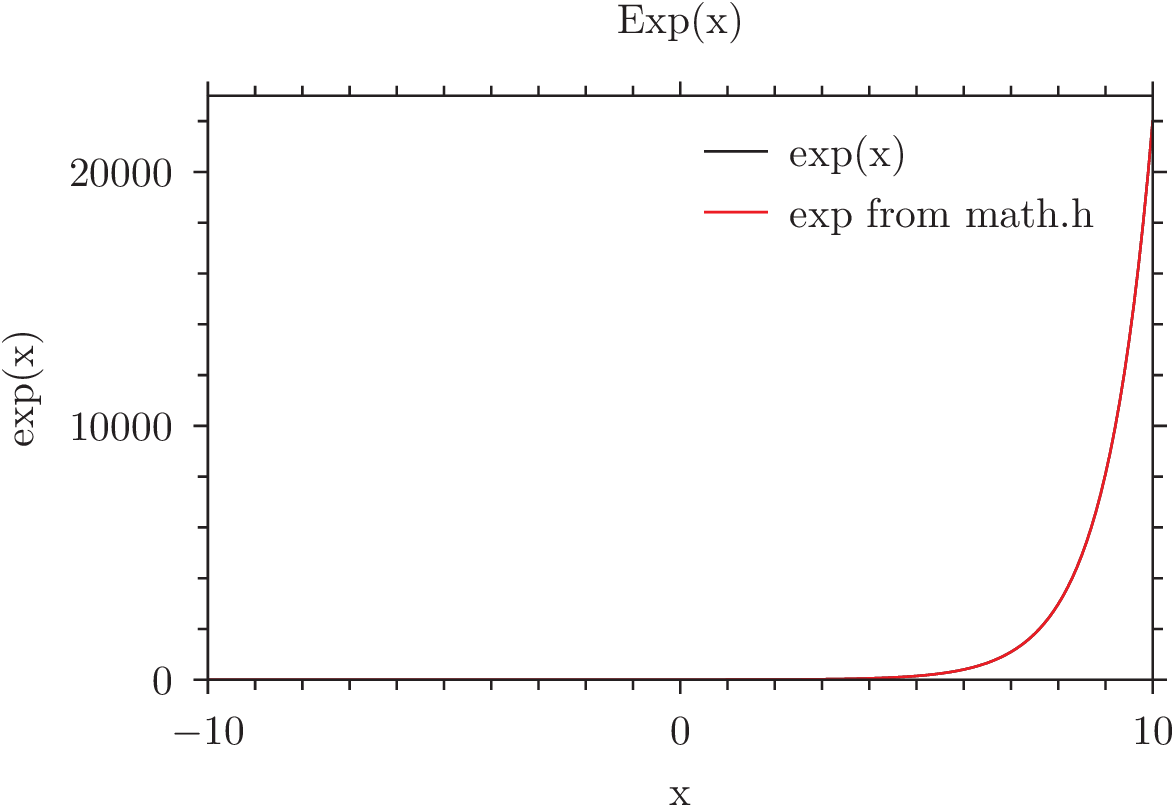
\includegraphics[width=70mm]{exp.png}
    \caption{A plot of the Taylor expansion of $\exp{x}$ of $x$ ranging from $-10$ to $10$ with stepsize of $1/10$. The value of $\exp{(x)}$ from math.h is plotted aswell.}
    \label{TaylorPlot}
\end{figure}
In figure \ref{TaylorPlot} the value of $\exp{x}$ from the Taylor expansion is plotted along with the computed value from $math.h$ with $x\in[-10,10]$. The two lines are equal to each other, suggesting that the Taylor expansion implemented works.\\\\
By removing the conditions written above the following plot is made
\begin{figure}[h!]
    \centering
    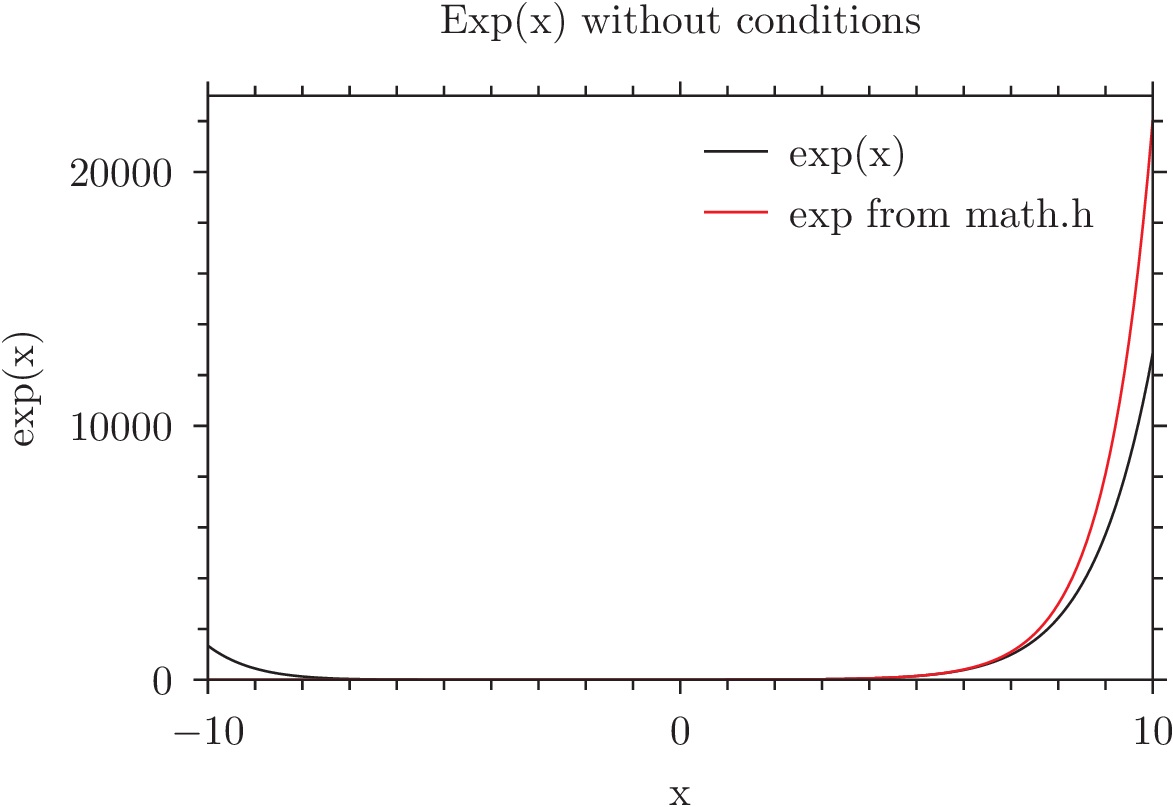
\includegraphics[width=70mm]{exp_wrong.png}
    \caption{A plot of $\exp{x}$ from the Taylor expansion (with conditions excluded) and the math.h lib.}
    \label{TaylorPlot_wrong}
\end{figure}
As seen in figure \ref{TaylorPlot_wrong} the Taylor expansion deviates from the calculated values of math.h with the lower returned values for $x>1./8$ and the incorrect increasing values for $x<0$.
\section*{Conclusion}
The implementation of the exponential function proved succesful when comparing it to the values given by math.h. The correct values computed is caused by the two conditions and the high order of the Taylor expansion. This suggests that higher orders merely would increase the computation time. 

\end{document}
